%! Author = javif
%! Date = 9/11/2023


\chapter{Results}\label{ch:results}

The implemented methodology led to the development of a system that possesses the ability to efficiently produce and
deliver static content.
This system is characterized by its user-friendly nature, requiring minimal effort to learn
and operate.
Furthermore, it is equipped with comprehensive logging capabilities, enabling users to gain insights into the
system's operations at any given time.

The first step to follow in order to use VaGo, is to install the software using the native Go command \emph{go install}.
This will get all the required dependencies, compile the code, build an executable and install the CLI for the system
to recognize it as a command-line tool.

Moreover, to perform the most basic tests, a markdown file with all the types of tokens has been used to make sure
everything is
being correctly parsed.
The file contains a structure similar to the following (whole file not included for simplicity), named as \emph{first
.md}:

\begin{code}

    ## Emphasis

    **This is bold text**

    __This is bold text__

    *This is italic text*

    _This is italic text_

    ~~Strikethrough~~


    ## Blockquotes


    > Blockquotes can also be nested...
    >> ...by using additional greater-than signs right next to each other...
    > > > ...or with spaces between arrows.


    ## Lists

    Unordered

    + Create a list by starting a line with `+`, `-`, or `*`
    + Sub-lists are made by indenting 2 spaces:
    - Marker character change forces new list start:
    * Ac tristique libero volutpat at
    + Facilisis in pretium nisl aliquet
    - Nulla volutpat aliquam velit
    + Very easy!

    Ordered

    1. Lorem ipsum dolor sit amet
    2. Consectetur adipiscing elit
    3. Integer molestie lorem at massa


    1. You can use sequential numbers...
    1. ...or keep all the numbers as `1.`

    Start numbering with offset:

    57. foo
    1. bar


    ## Code

    Inline `code`

    Indented code

    // Some comments
    line 1 of code
    line 2 of code
    line 3 of code
    .
    .
    .
\end{code}


This way, it can be used to test the parsing and generation mechanism.
Adding this file to the input file, and using the following configuration (\emph{config.yaml}), the building process
can be
started.

\begin{code}
    # config.yaml

    input: "./source/"
    template: "./template/index.html"
    output: "./out/"
\end{code}


Where \emph{./source/} is the input folder where the markdown file is stored, \emph{./out/} is the output folder
where the result will be saved, and \emph{./template/index.html} is the template file with the following structure:

\begin{code}

<!DOCTYPE html>
<html lang="en">
<head>
<meta charset="UTF-8">
<link rel="stylesheet" href="styles.css">
<title> {{ .H1 }} </title>
</head>
<body>

<section> {{ .Content }} </section>

</body>
</html>
\end{code}

The template structure is rather simple, but it serves the purpose of testing the parsing mechanism.
It's important to note that the \emph{.Content} variable is being used, meaning that all the content will be displayed
in one single place, without much customization.


Then, the Build process is executed by using the command \emph{vago build}.
This will start the parsing process, displaying logs of every steps, and finally the new file generation will be
performed to create an HTML version file of the provided input, following the given template.

\begin{figure}
    \centering
    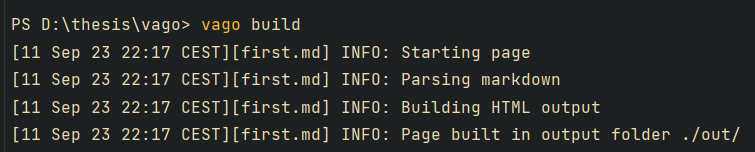
\includegraphics[width=1\textwidth]{/results/vagobuild}
    \caption{VaGo build execution with first.md}
    \label{fig:figure}
\end{figure}

Now, inspecting the \emph{/out/} folder, a new file can be seen with the same name as the input file, but with the
HTML extension: \emph{first.html}.
Reviewing the content of this file, it can be verified that it has been correctly parsed, as each token is correctly
mapped to its equivalent HTML tag (whole file not included for simplicity):

\begin{code}
<section>
<h2>
    Blockquotes</h2>
    <p><strong>This is bold text</strong></p>
    <p><strong>This is bold text</strong></p>
    <p><em>This is italic text</em></p>
    <p><em>This is italic text</em></p>
    <p><del>Strikethrough</del></p>

    </section>



    <section>
    <h2>Lists</h2>
    <blockquote>
    <p>Blockquotes can also be nested&hellip;</p>

    <blockquote>
    <p>&hellip;by using additional greater-than signs right next to each other&hellip;</p>

    <blockquote>
    <p>&hellip;or with spaces between arrows.</p>
    </blockquote>
    </blockquote>
    </blockquote>

    </section>



    <section>
    <h2>Code</h2>
    <p>Unordered</p>
    <ul>
    <li>Create a list by starting a line with <code>+</code>, <code>-</code>, or <code>*</code></li>
    <li>Sub-lists are made by indenting 2 spaces:

    <ul>
    <li>Marker character change forces new list start:

    <ul>
    <li>Ac tristique libero volutpat at</li>
    <li>Facilisis in pretium nisl aliquet</li>
    <li>Nulla volutpat aliquam velit</li>
    </ul></li>
    </ul></li>
    <li>Very easy!</li>
    </ul>
    <p>Ordered</p>
    <ol>
    <li><p>Lorem ipsum dolor sit amet</p></li>

    <li><p>Consectetur adipiscing elit</p></li>

    <li><p>Integer molestie lorem at massa</p></li>

    <li><p>You can use sequential numbers&hellip;</p></li>

    <li><p>&hellip;or keep all the numbers as <code>1.</code></p></li>
    </ol>
    <p>Start numbering with offset:</p>
    <ol>
    <li>foo</li>
    <li>bar</li>
    </ol>

    </section>



    <section>
    <h2>Tables</h2>
    <p>Inline <code>code</code></p>
    <p>Indented code</p>
    <pre><code>// Some comments
    line 1 of code
    line 2 of code
    line 3 of code
    </code></pre>
\end{code}


Nonetheless, in order to verify that it's working as expected with all the tags correctly set, it is imperative to test
it out in a browser, to determine if the content is being displayed as it should.
Therefore, this can be tried out by simply starting a server and accessing this file using URL path \emph{/first.html}.
On a side note, the home page is not being set in the configuration file, hence the server will lack of a homepage,
although it doesn't impose an issue for the purpose of this test.
The test can be started by using the command \emph{vago serve}:

\begin{figure}
    \centering
    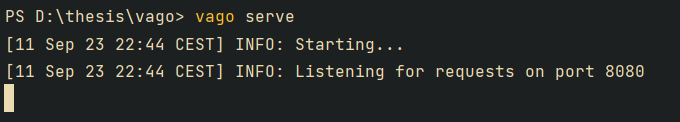
\includegraphics[width=1\textwidth]{/results/vagoserve}
    \caption{VaGo serve execution with first.md}
    \label{fig:serve}
\end{figure}


Then, accessing \emph{localhost:8080/first.html} the following page can be seen in the browser:

\begin{figure}
    \centering
    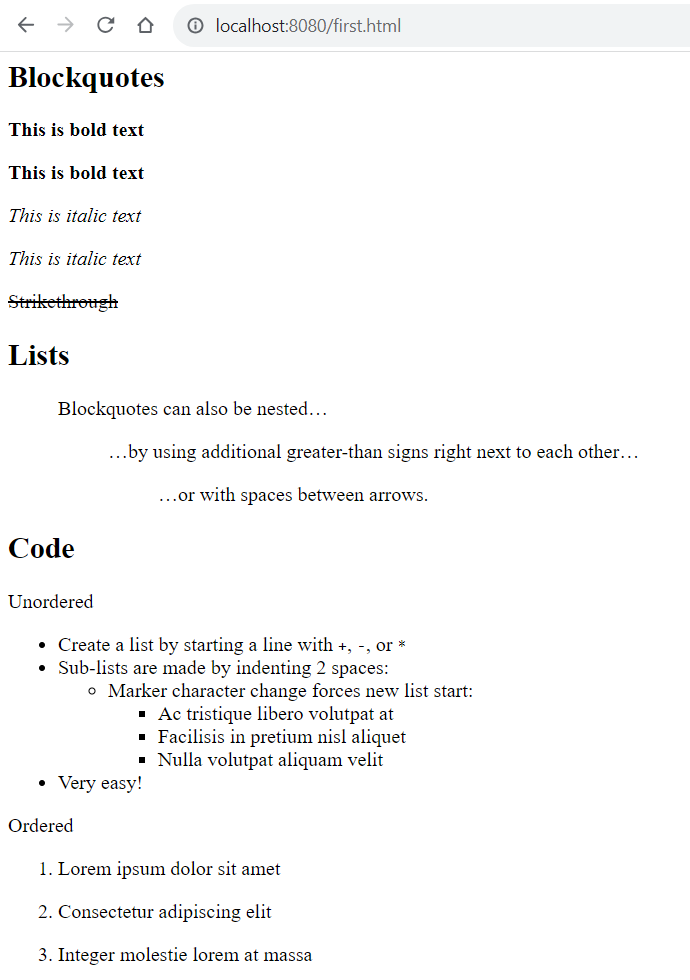
\includegraphics[width=0.8\textwidth]{/results/browserfirsthtml}
    \caption{first.html displayed in browser.}
    \label{fig:browserfirst}
\end{figure}

With this simple test, the main functionality of parsing, generating, serving and routing has been successfully
demonstrated, proving VaGo to be a static site generator capable of performing the most simple tasks.

Notwithstanding, there is left to try the templating and theming system, to ensure its flexibility capabilities.
For this, a new input file is constructed with several sections divided by titles.
The new file will be named as lorem.md, and it has the following structure (not all the content is displayed for
simplicity):

\begin{code}

    # Lorem Ipsum

    ## What is Lorem Ipsum?

    Lorem Ipsum is simply dummy text of the printing and
    typesetting industry. Lorem Ipsum has been the industry's
    standard    dummy text ever since the 1500s, when an
    unknown printer took a galley of type and scrambled it
    to make a type specimen book. It has survived not only
    five centuries, but also the leap into electronic
    typesetting, remaining essentially unchanged. It was
    popularised in the 1960s with the release of Letraset
    sheets containing Lorem Ipsum passages, and more
    recently with desktop publishing software like Aldus
    PageMaker including versions of Lorem Ipsum.

    ## Why do we use it?

    It is a long established fact that a reader will be
    distracted by the readable content of a page when
    looking at its layout. The point of using Lorem
    Ipsum is that it has a more-or-less normal
    distribution of letters, as opposed to using
    'Content here, content here', making it look like
    readable English. Many desktop publishing packages
    and web page editors now use Lorem Ipsum as their
    default model text, and a search for 'lorem ipsum'
    will uncover many web sites still in their infancy.
    Various versions have evolved over the years,
    sometimes by accident, sometimes on purpose
    (injected humour and the like).

\end{code}

Since the content of this new input file has defined sections, the previous template can be modified to take advantage
of this and provide a more customized structure, iterating over second headings \emph{H2} and using the same index to
iterate over \emph{P} values.
This is done by using the \emph{range} function from Go templates and storing a
reference to \emph{P} to avoid losing its content within the range context, then providing the same iterator
\emph{\$i} on the function \emph{index}.

These functionalities are all part of the native Go template system, so VaGo takes advantage of the extended already
provided features to provide flexible customization options.

\begin{code}
<!DOCTYPE html>
<html lang="en">
<head>
<meta charset="UTF-8">
<link rel="stylesheet" href="styles.css">
<title> {{ .H1 }} </title>
</head>
<body>

<h1> {{ .H1 }} </h1>
{{ $p := .P }}
{{
    range $i, $H2 := .H2 }}

<section>
<h2>{{ $ H2 }}</h2>
{{ index $p $i }}
</section>

{{ end }}

</body>
</html>
\end{code}

In the same way, a new CSS file is added to the \emph{/styles/} folder, making use of the theme variables that will be
defined later:

\begin{code}
section{
background-color: {{ .background }};
margin: {{ .margin }};
padding:  {{ .padding }};
}
\end{code}

Following this, the variables \emph{background, margin, padding} are defined in the \emph{theme.yaml} file, and
further users can modify these variables to match their styling needs. For the moment, the content of this file will
be the following:

\begin{code}
background: "#696969"
margin: "5px"
padding: "5px"
\end{code}

Consequently, a few modifications to the configuration file (config.yaml) are required to add the new theme, and the
new file \emph{lorem} is added as a homepage too, in order to try out the home page feature.

\begin{code}
input: "./source/"
template: "./template/index.html"
output: "./out/"

# Theme:
styles: "./styles/"
theme: "./theme.yaml"

home: "lorem.html"
\end{code}

Once everything is set up, a new building process can be started using the same command \emph{vago build}, and this
will provide context on the files parsed and created, including the style files.

\begin{figure}
\centering
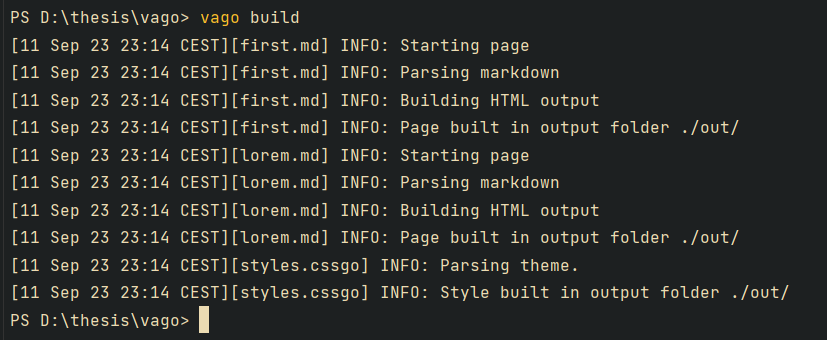
\includegraphics[width=1\textwidth]{/results/vagobuild2}
\caption{Building with new file, template and theme.}
\label{fig:build2}
\end{figure}

After this, the files \emph{lorem.html} and \emph{styles.css} has been added to the output folder \emph{/out/}.
Then, to verify the web content and its new styles added, a new server has to be started using the same command
\emph{vago serve} (output omitted for simplicity).
Following, the URL \emph{localhost:8080} is accessed, and the content of lorem.html is correctly displayed as home
page, with a set of styles provided as expected:

\begin{figure}
\centering
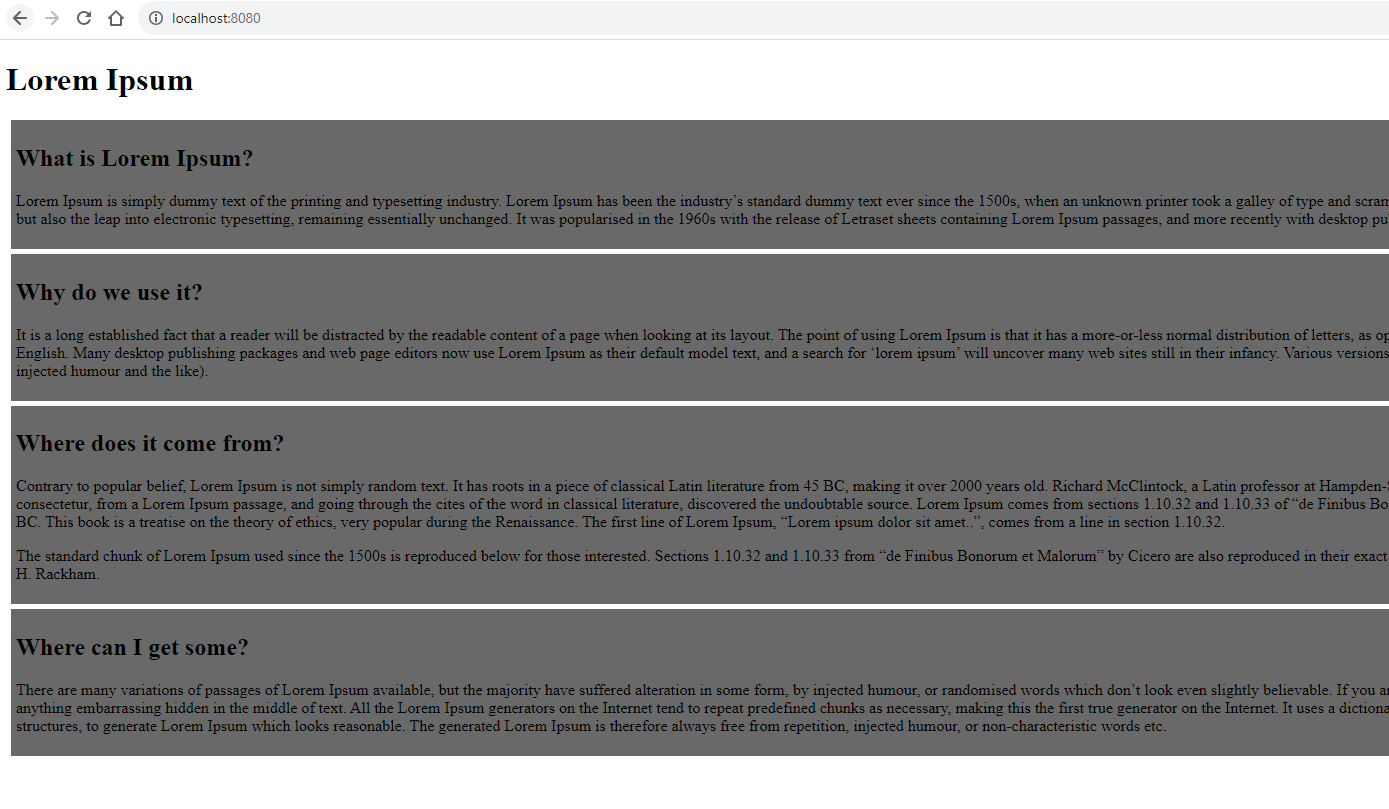
\includegraphics[width=1\textwidth]{/results/vagoserve2}
\caption{Serving lorem.html as homepage with styles.}
\label{fig:serve2}
\end{figure}

The provided color scheme and separation between sections may not be desirable. However, this can be easily modified
by accessing the theme file and adding the desired characteristics. A cyan like color should provide better
readability, and an increased margin and padding should be enough to split the sections.

\begin{code}
background: "#C0FFEE"
margin: "18px"
padding: "24px"
\end{code}

After building and starting the server once again (ouput omitted for simplicity), the following content is displayed in
the browser:

\begin{figure}
\centering
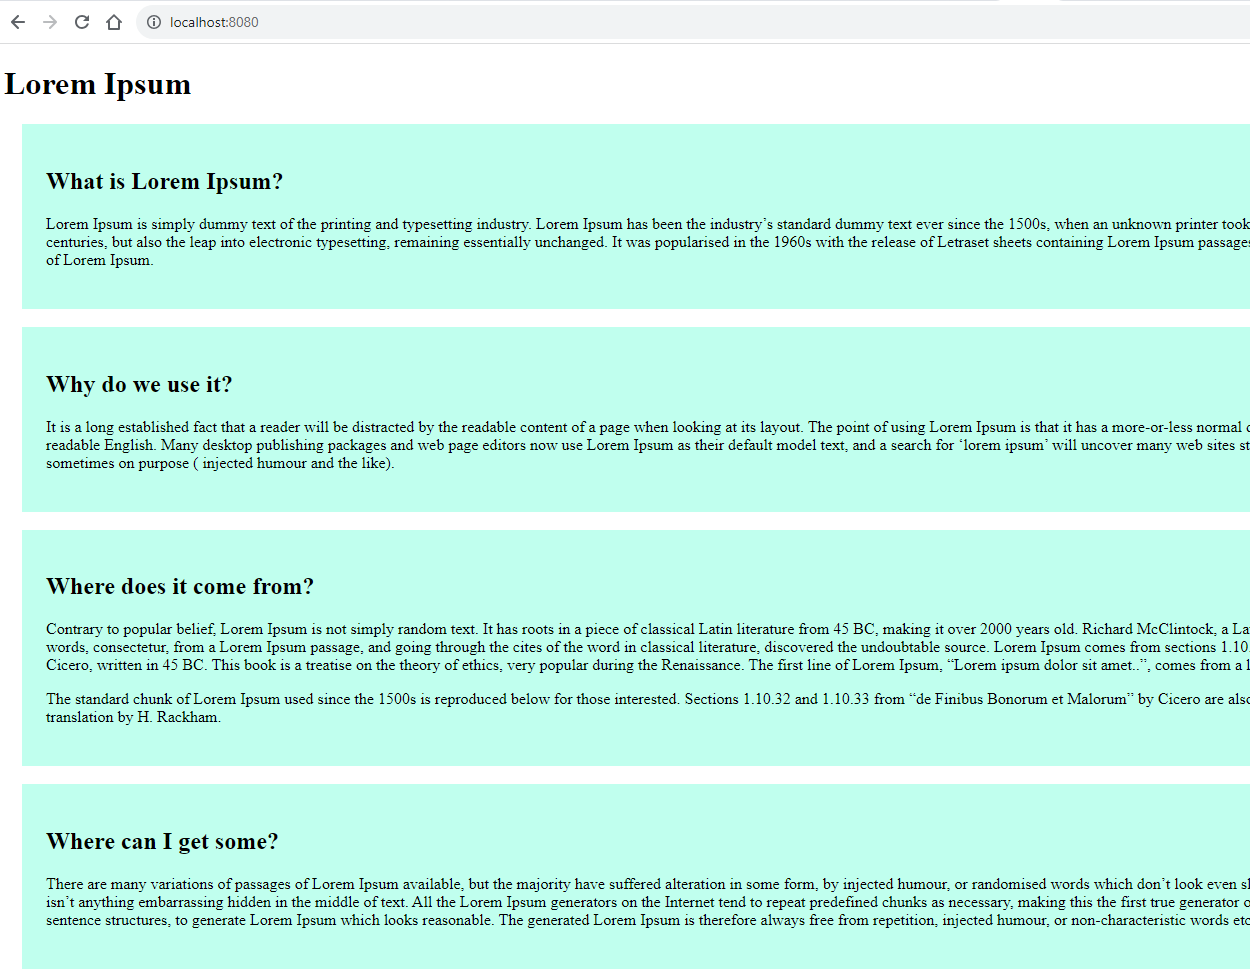
\includegraphics[width=1\textwidth]{/results/vagoserve3}
\caption{Serving lorem.html after modifying the theme.}
\label{fig:serve3}
\end{figure}